% !Mode:: "TeX:UTF-8"
% !TEX program  = xelatex
\section{绪论}



\subsection{背景}
21世纪以来,机器人在生产生活中扮演越来越重要的角色。现代机器人是由遥操作演变而来,首先问世的是固定基座的机器人,也就是机械臂,随后才出现了移动机器人\cite{corke2011robotics}。移动机器人运用广泛,包括地面、水下、控制乃至外太空\cite{Siciliano2016handbook}。地面移动机器人则在物流、货物搬运、探索、巡逻等室内外环境有许多用途。

\begin{figure}[h!]
  \centering
  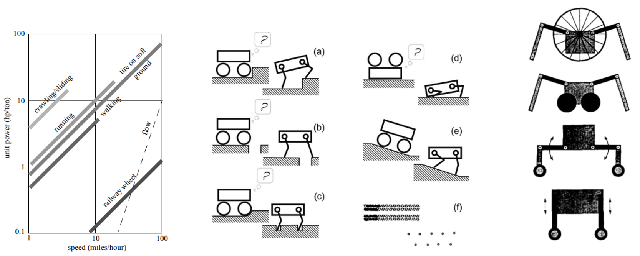
\includegraphics[width=1.0\linewidth]{figures/Sec1/wl.png}
  \caption{
  不同类型的移动(locomotion)效率对比\cite{siegwart2011introduction}(左),与轮式机器人与腿式机器人的通过性对比\cite{siegwart2011introduction}(中),与轮腿独立和轮腿共融的示意图\cite{eiji1993leg}(右)。
  }
  \label{fig:sec1-wl}
   \vspace{6pt}
\end{figure}

主流的地面移动机器人往往是轮式或者腿式,轮式机器人(Wheeled Robot)在平地上效率极高,且其机械结构简单,可靠性好,易于控制,率先得到了快速的发展与广泛的运用。结合一些感知与规划的算法,轮式机器人已经广泛运用在生产生活中,如无人工厂AGV\cite{Siciliano2016handbook}\cite{khatib2016springer}(Auto Guided Vehicle,自动引导车辆),无人码头的集装箱运转车辆\cite{Qingdaoport}和在家庭中常见的扫地机器人,甚至近些年来得以迅速发展的无人驾驶车辆。但面对一些复杂的非结构化环境下的任务,如在具有楼梯的建筑物内巡检,或在废墟中救援等等,传统的轮式移动机器人已经难以满足实际应用的需求。这些场景或者是为人类生产生活所设计的,如梯子、楼梯,有些则对于人类也充满挑战,如废墟等等。轮式机器人需要在平整的地面上才能发挥出速度快、效率高的优势,但在这些场景则会卡在障碍物中或无法上下楼梯,因而无法完成任务(如图\ref{fig:sec1-wl}中所示)。

而腿式机器人(Legged Robot)具备在复杂非结构化环境中更好的机动性和适应性,尤其是双足腿式机器人(Biped Legged Robot),其落地点可以在一定范围内选取,且腿可以实现一种类似于主动悬挂的效果\cite{Raibert1984walkingrobots}(如图\ref{fig:sec1-wl}中所示),非常适合在为人类设计的环境中工作\cite{Yamaguchi1997humanoid}。但腿式机器人移动速度慢,能量消耗高(如图\ref{fig:sec1-wl}左所示),且双足机器人控制困难。相比于轮式机器人,腿式机器人须要拥有更多自由度,且关节扭矩大,因此对驱动系统和机械设计提出很高要求。双足机器人的运动控制须考虑其平衡,且须规划落脚点,然后控制各个关节,规划及运动控制难度和复杂度都远超轮式机器人,且在运动速度远不及轮式机器人的情况下,消耗的能源也远超轮式机器人。

双足轮腿机器人(Bipedal Leg-wheeled Robot,以下简称轮腿机器人)结合了轮式机器人的高速高效性和腿式机器人对复杂地形的适应性强的特点,增大机器人作业范围和环境适应性,这些机器人在平地上使用轮子移动,遇到障碍物时则跳过或跨过障碍物(如图\ref{fig:sec1-wl}右所示)。轮腿共融机器人的两侧的腿可以独立改变长度,使得机器人通过性、机动性更好,能在狭小空间中运动,转弯时保持高速,还能在不平整地面保持平衡。当然,轮腿机器人也结合了轮式和腿式的其他特点,其控制复杂度比轮式高,但却不需要像腿式机器人一样需要规划落脚点和步态,因此难度比腿式机器人低。正因为结合了轮式与腿式的优点,轮腿机器人近年来得到了广泛的发展。

\subsection{国内外研究现状}

国外的Boston Dynamics的Handle机器人(图\ref{fig:sec1-Handle})在物流、仓储方面表现出令人惊叹的稳定性、灵活性和效率,但是Boston Dynamics并未发表论文公开其背后的机械设计及控制算法等。据开源资料披露,其移动速度可达24km/h,远超过该公司的双足机器人Atlas 5km/h的速度。Handle物流机器人拥有一个巨大的“动力尾”,笔者推测其液压动力系统和电池等安装在其中。根据Boston Dynamics展示的视频信息,Handle机器人在加减速和拿起货物的时候,“动力尾”会主动运动以辅助机器人保持平很,以提升机器人的整体性能。

\begin{figure}[h!]
  \centering
  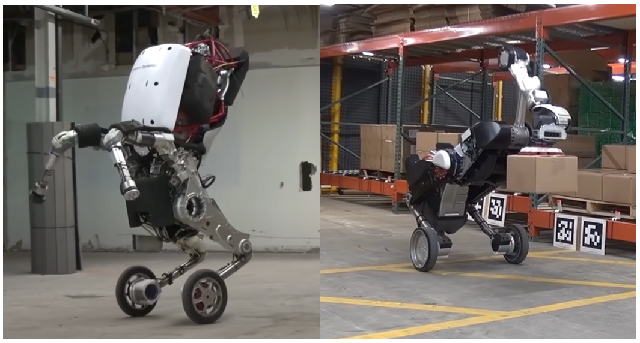
\includegraphics[width=0.5\linewidth]{figures/Sec1/Handle.png}
  \caption{
  Boston Dynamics的第一代\cite{introducinghandle}(左)和第二代\cite{handle4logistics}(右)Handle机器人
  }
  \label{fig:sec1-Handle}
   \vspace{6pt}
\end{figure}

ETH的Ascento(图\ref{fig:sec1-Ascento})机器人发表了论文,介绍了其使用场景、机械设计和控制算法,其主要应用场景为探索、监控、巡查,其腿部仅有一个自由度,并经过拓扑优化设计四杆机构,使得电机可以控制机器人质心近似上下移动,从而实现跳跃功能。其跳跃功能是为了上楼梯涉及的,后来Ascento机器人被开发用于巡逻与探索,且推出专业版(图\ref{fig:sec1-AscentoPizza})。普通的Ascento机器人其鲜有搭载负载的场景,考虑到其轮腿设计,安装负载时必须使其质心与机器人与地面接触点连线竖直,如图\ref{fig:sec1-AscentoPizza}所示。Ascento专业版机器人采用了悬吊的方式装载重物,但其没有发表论文或公开资料,因此实际性能并未可知。Ascento机器人的2019年iCRA\cite{klemm2019ascento}论文主要提出了基于多个参数插值的LQR平衡方式,同时通过调试的方式实现了摔倒-站立和定高度跳跃,然后在2020RAL\cite{klemm2020lqr}期刊中运用了全身力控,进一步增强了稳定性和抗扰能力。

\begin{figure}
  \centering
  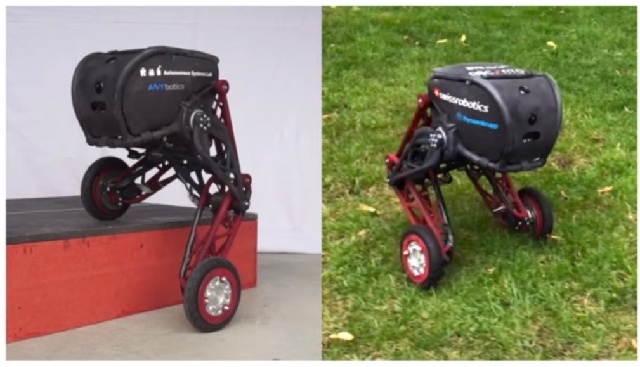
\includegraphics[width=0.5\linewidth]{figures/Sec1/Ascento.png}
  \caption{
  ETH的Ascento机器人\cite{klemm2019ascento} \cite{klemm2020lqr}
  }
  \label{fig:sec1-Ascento}
   \vspace{6pt}
\end{figure}

\begin{figure}
  \centering
  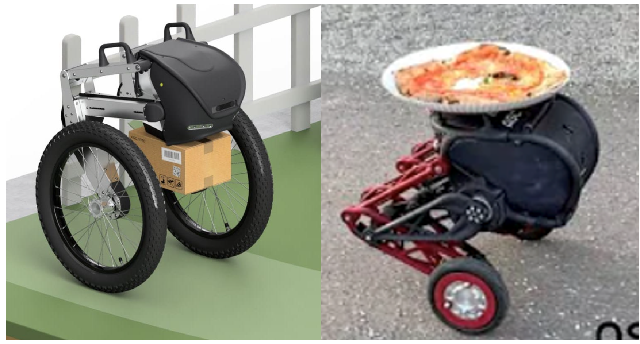
\includegraphics[width=0.5\linewidth]{figures/Sec1/AscentoPizza.png}
  \caption{
  Ascento专业版\cite{ascentopro}机器人运送货物时,将货物吊装在机体下方(左),Ascento机器人运送货物时,需调整货物位置(右)
  }
  \label{fig:sec1-AscentoPizza}
   \vspace{6pt}
\end{figure}


哈尔滨工业大学的WLR机器人(图\ref{fig:sec1-HITWRL})尺寸与Handle机器人接近,其同样采用液压驱动 ,使用金属3D打印作为液压动力输送管道,但其动力源是外置的,且机器人尺寸较大,因此并不适用于室内环境进行家庭服务等工作。

\begin{figure}[h!]
  \centering
  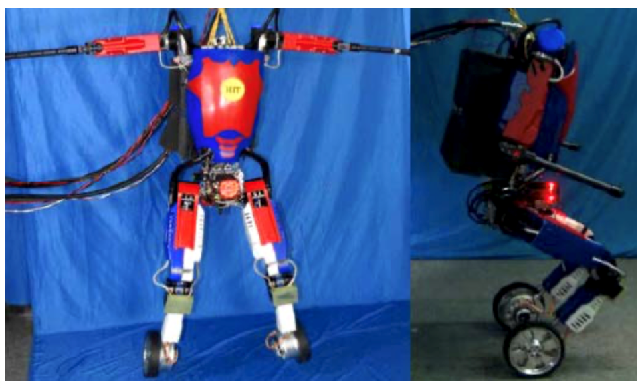
\includegraphics[width=0.5\linewidth]{figures/Sec1/HITWRL.png}
  \caption{
  哈尔滨工业大学的WLR机器人\cite{li2018design}
  }
  \label{fig:sec1-HITWRL}
   \vspace{6pt}
\end{figure}

腾讯的Ollie机器人(图\ref{fig:sec1-Ollie})采用了五杆机构设计的腿部结构,与传统的双足足式机器人有较大差别。五杆机构属于并联机构,因此可以获得扭矩叠加的效果,从而优化跳跃表现,但并联机构也带来了解算复杂、工作空间小的缺点。此外,Ollie机器人还设计有一个安装了万向轮的尾巴,类似于Handle物流机器人的动力尾,在Ollie展示其“翻跟斗”的能力时,尾巴很好的辅助其完成旋转一周的动作,但据Ollie披露的视频显示,尾巴仅在此发挥作用,其余时间均收起,与身体保持固连的状态。

\begin{figure}[h!]
  \centering
  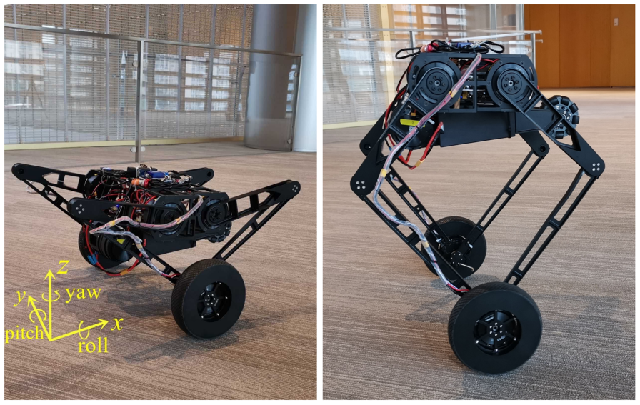
\includegraphics[width=0.5\linewidth]{figures/Sec1/Ollie.png}
  \caption{
  腾讯的Ollie机器人\cite{wang2021balance}
  }
  \label{fig:sec1-Ollie}
   \vspace{6pt}
\end{figure}

南方科技大学的哪吒(NeZha)机器人(图\ref{fig:sec1-sr600nezha})在控制上体现出强大的稳定性与鲁棒性,并首次提出了轮腿机器人跳跃的综合规划与控制策略\cite{chen2020underactuated},并在仿真中得到了验证。

\begin{figure}[h!]
  \centering
  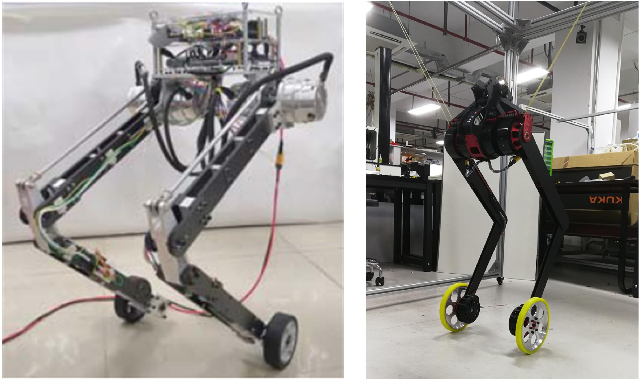
\includegraphics[width=0.5\linewidth]{figures/Sec1/sr600nezha.png}
  \caption{
  哈尔滨工业大学(深圳)的SR600机器人\cite{zhang2020sr600}(左)和南方科技大学的哪吒机器人(右)
  }
  \label{fig:sec1-sr600nezha}
   \vspace{6pt}
\end{figure}

哈尔滨工业大学(深圳)的SR600机器人(图\ref{fig:sec1-sr600nezha})采用了QDD\cite{wensing2017proprioceptive}(Qausi-Direct Drive,准直驱)的膝关节和髋关节电机,但采用有刷电机作为轮子驱动器,且经过减速箱、弹性联轴器与锥齿轮传动,无法实现力透传,且其QDD电机减速比过大。该机器人实现了静态平衡\cite{zhang2019system},并在仿真中实现了变高度平衡\cite{liu2019dynamic}。

\subsection{研究内容和系统框架}
本毕业设计希望能实现设计搭建类似于Ascento机器人的样机。Ascento使用单自由度四连杆机构,通过优化杆长实现近似上下运动。与之不同的是,本毕设使用双电机设计,从而在运送货物时无须调整其位置,使得整体布局更接近SR600机器人的设计。本毕设的目标场景是,在为人类设计的室内环境中,机器人能前往该环境的所有地点。相比于Handle机器人和WLR机器人,本毕设采用的方案成本更低、更易于实现,可以推广到家庭、餐馆、医院服务等无须大载重,但对机器人尺寸、灵活度要求较高的场景。Ascento虽然实现了全身控制\cite{klemm2020lqr},但其自由度偏少,而SR600虽然使用了QDD电机,但其减速比过高(60:1,甚至不符合文献\cite{wensing2017proprioceptive}中要求的减速比不大于36:1),且轮子电机及相关传动、减速无法实现力控。本毕业设计的创新点在于,全部采用减速比在10:1之内的QDD电机,实现效果更好的QDD力控,因而可以为后续基于此平台实现全身控制及跳跃做准备。

\begin{figure}[t!]
  \centering
  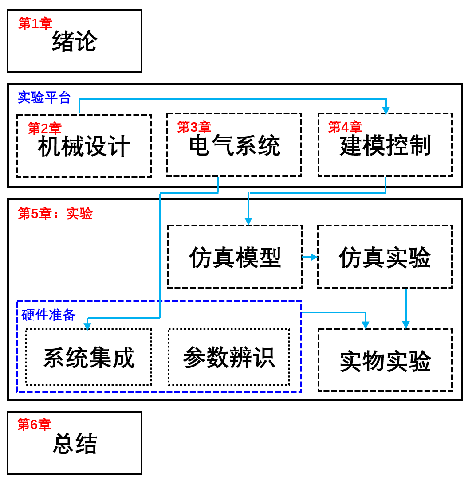
\includegraphics[width=0.7\linewidth]{figures/Sec1/frame1.png}
  \caption{
  论文各章节主要内容
  }
  \label{fig:sec1-frame1}
   \vspace{4pt}
\end{figure}

本毕设将先分析将要设计的轮腿机器人的结构并基于此展开机械设计,然后将QDD电机和驱动器、电池、计算平台运用并布置其中。根据机械设计,本毕设将对机器人进行等效、简化的建模。将建立运动学模型一遍调试及是实现简单的控制,建立动力学模型以了解系统特性,并依次设计若干控制器。本毕设将首先设计简单的控制器,以验证整套硬件系统,然后更换为复杂但效果更好的控制器。同时会根据机械设计与建模结果搭建仿真模型,并在仿真中测试控制器,进行仿真实验。为将上述控制器迁移到实物中,需要进行硬件准备。本毕设将根据电气系统中选用的各部件进行联调,实现系统集成的效果,然后对机器人本体进行参数辨识,以更正仿真模型中使用CAD(Computer Assistant Design,计算机辅助设计)模型估算的各种误差。最终,通过仿真验证的控制器将会迁移到通过硬件准备的实物上,进行实物实验。

本毕设论文的组织形式如图\ref{fig:sec1-frame1}所示,考虑到本毕设的目的是设计与制作实验平台,并运用控制算法,因此第二章、第三章和第四章分别从机械设计、电气系统和建模控制的角度介绍。为验证本毕设设计制作的轮腿机器人的实际效果,需要进行实验,包括仿真实验和实物原型机实验。在进行仿真实验之前,需要进行仿真模型搭建,而进行实物实验之前,需要对硬件平台进行准备,如电气系统集成和参数辨识等。

本毕业论文的包括的主要内容及主要的贡献点如图\ref{fig:sec1-frame2}所示,也分别对应每个章节的相应内容。

\begin{figure}[h!]
  \centering
  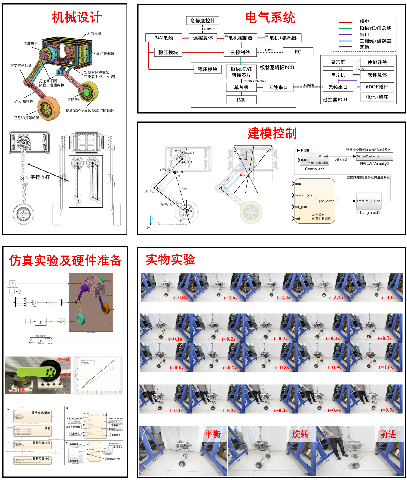
\includegraphics[width=0.9\linewidth]{figures/Sec1/frame2.1.png}
  \caption{
  论文总体框图
  }
  \label{fig:sec1-frame2}
   \vspace{4pt}
\end{figure}

\subsection{本章小结}
本章中,介绍了轮腿机器人结合了轮式机器人和腿式机器人的优点,以及国内外的相关研究现状。然后介绍了本文的研究内容和研究框架,最终本毕业设计的最终实物如图\ref{fig:sec1-result}所示。

\begin{figure}[t]
  \centering
  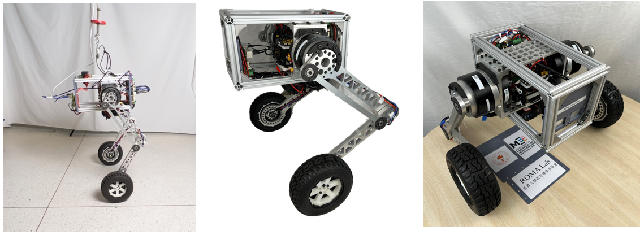
\includegraphics[width=1.0\linewidth]{figures/Sec1/result.png}
  \caption{
  本毕业设计最终实现的轮腿机器人原型机示意图
  }
  \label{fig:sec1-result}
   \vspace{4pt}
\end{figure}